\documentclass[10pt,conference,compsocconf]{IEEEtran}

\usepackage{hyperref}
\usepackage{graphicx}	% For figure environment


\begin{document}
\title{Machine Learning Report}

\author{
  Raphael Barman, Hakim Invernizzi, Rehan Mulakhel\\
  \textit{EPFL students}
}

\maketitle

\begin{figure}
\begin{center}
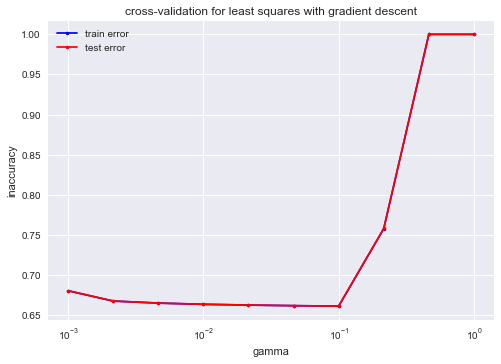
\includegraphics[width=4.5cm]{cross_validation_least_squares_GD.png}
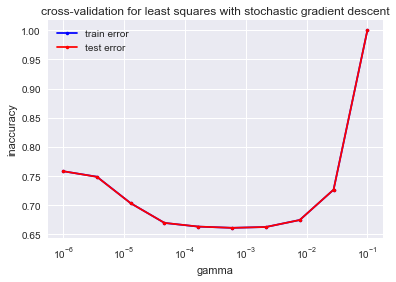
\includegraphics[width=4.5cm]{cross_validation_least_squares_SGD.png}
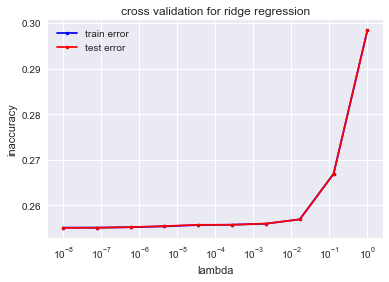
\includegraphics[width=4.5cm]{cross_validation_ridge_regression.png}
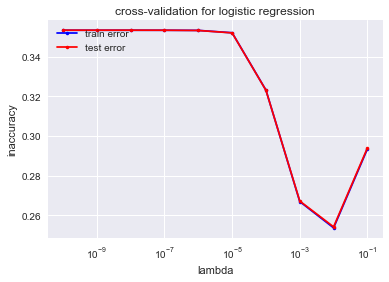
\includegraphics[width=4.5cm]{cross_validation_logistic_regression.png}
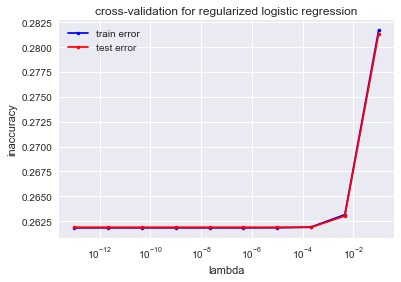
\includegraphics[width=4.5cm]{cross_validation_reg_logistic_regression.png}
 \end{center}
 \begin{center}
 \caption{\label{fig:figure1}Result of Cross-Validation with 10 folds. On the X-axis we have the ML method parameter to be tuned, on the Y-axis a measure of the inaccuracy. From top to bottom: (a) least squares GD (b) least squares SGD (c) ridge regression (d) logistic regression (e) logistic regression with regularization}
 \end{center}
\end{figure}

\section{Part I: Machine learning methods implementation}
We start by the description of our implementation of the six machine learning methods.

Please note that we have defined our own metric to estimate prediction error, which
is not the MSE but simply the percentage of incorrectly predicted outputs, which
we call inaccuracy.
This metric is used exclusively to evaluate performance and is not part of the
implementation.

All the results presented have been found with a 10-fold cross-validation.

\subsection{Linear regression using gradient descent}
The implementation is simple: we update iterating the initial weight by subtracting a pondered gradient.
Figure \ref{fig:figure1} (a) shows the cross-validation results with 500
iterations and gamma taking values in the range $[10^{-3}, 10^{0}]$ with step
$10$. It can be noted that the method gives around 66\% inaccuracy in the best
case, and performs best when gamma is on the order of $10^{-1}$. This quite bad
performance can be explained by the fact we iterate only 500 times, thus
the gradient descent may not have converged. However, more iterations are costly
because the gradient costs $O(N\cdot D)$ to compute.

\subsection{Linear regression using stochastic gradient descent}
The difference compared to the previous method is that at each iteration a
random sample is chosen in order to
create size-1 batches. The gradient is then computed, pondered and used to
update the weight. Figure \ref{fig:figure1} (b) shows the cross-validation
results with 10,000 iterations and gamma taking value in the range $[10^{-6},
10^{-1}]$ with step $10$. it can be noted that the method also gives $66$\%
inaccuracy in the best case, and performs best when gamma is on the order of
$10^{-3}$. The result is coherent with the theory, a stochastic gradient descent
is cheap to compute, however with a batch of size $1$, it has a tendency to have a
lot of variance and to be slow to converge.

\subsection{Least squares regression}
The pseudo-inverse of the feature matrix $tx$ is computed and then multiplied with the classification vector $y$ to obtain the weight.
The inaccuracy is about $25.5$\% for both train and test data set. The result
is coherent, it is the least square solution, however, it is costly to compute.

\subsection{Ridge regression}
The weight is computed by solving the ridge regression equation, yielding $w = (X^{T}X + \lambda'I)^{-1}X^{T}y$.
Figure \ref{fig:figure1} (c) shows the cross-validation results with lambda taking values in the range $[10^{-8}, 10^{0}]$ with step $10$. It can be noted that the performance of the ridge regression is comparable to that of the simple least square regression, suggesting that regularization applied to the whole data set provides little improvement. This might mean that the problem is well-conditioned, or in other words that the model isn't over- nor under-fitting.

\subsection{Logistic regression}
The weight is updated by subtracting a gradient whose ponderation takes into % TODO: "ponderation" is not an English word?
account its hessian matrix. Figure \ref{fig:figure1} (d) shows the
cross-validation results with $10,000$ iterations and gamma taking values in the
range $[10^{-10}, 10^{-1}]$ with step $10$. It can be noted that method gives
around $25.7$\% inaccuracy in the best case. This gives a much better result than
the linear regression with gradient descent, which is coherent since we have
indeed a binary classification problem.

\subsection{Regularized logistic regression}
Logistic regression with the addition of a penalty term to account for linearly separable data. Figure \ref{fig:figure1} (e) shows the cross-validation results with $10,000$ iterations, gamma on the order of $8 \cdot 10^{-3}$ and lambda taking values in the range $[10^{-10}, 10^{-1}]$ with step $10$. In can be noted that the method gives around $26.25$\% inaccuracy in the best case, reinforcing what previously said about regularization.

\section{Our Model}
\subsection{Exploratory Data Analysis and Feature Processing}
\subsubsection{Null values}
The presence of null values is well defined and allowed us to separate the
data set in 6 groups. We have noticed that all null values could be
explained by the the number of jet (\texttt{PRI\_jet\_num}) and by the presence or not of a
measure for the mass (\texttt{DER\_mass\_MMC}), thus we have created 6 groups, for number of jet
$\lbrace 0, 1, 2-3 \rbrace$ and the presence or not of mass measure. % TODO: why minus in the set?

\subsubsection{Percentiles}

By looking at the $95$\textsuperscript{th} percentile and the maximum values of each feature, we see
that in most cases, there are certainly a lot of outliers in some features.

\subsubsection{Histograms}

We have used histograms to have an idea of the underlying distribution.

Using the histograms, we see that the features related to \texttt{phi} have an uniform
distribution that is the same for \texttt{signal} and for \texttt{background}, this could mean
that these features do not add any relevant information for the classification.

We have also noticed some features have a long tail or are exponential, thus it could be a good
idea to log-normalize theme before using them.

\subsection{ML method and Cross-validation}
We have chosen to use Ridge Regression as the baseline since it has the lowest
inaccuracy.
All inaccuracy results that are given have been made on a 10-fold cross validation
using Ridge Regression. The baseline, i.e. Ridge Regression on a ten-fold, is
of inaccuracy $0.255152$ with $\lambda = 10^{-10}$
We will now explore five different ways of improving the baseline.

\subsubsection{Group separation}
Using the above observation, we have split the data set in $6$ groups. Hoping
the algorithms would find a better approximation of the underlying distribution
since we do not have to deal with null values. We have noticed an
improvement over the baseline: an inaccuracy of $0.234424$ with $\lambda =
10^{-10}$.

\subsubsection{Percentile cut}
We have tried to remove all values above a certain percentile and replace them with
the percentile, in order to delete all outliers and allowing to have a less
complex model. Using the 95th percentile, we have obtained an improvement: an
inaccuracy of $0.248784$ with $\lambda = 10^{-10}$

\subsubsection{Log-normalization}
Since some features have the shape of power laws and/or exponential, we have tried to
log-normalize where possible (we applied log on any value $>0$ in these
features). However, it has not resulted in an improvement over the baseline, with
an inaccuracy of $0.2618$ with $\lambda = 10^{-10}$. This could be explained by
the need of keeping the same distribution shape in order to be able to
differentiate \texttt{signal} and \texttt{background}.

\subsubsection{Removing features}
Since we have noticed the shape of all features related to \texttt{phi} are uniforms,
we have tried to remove those features in order to reduce the model complexity. We
have got a slight improvement, with an inaccuracy of $0.252068$ and $\lambda =
10^{-10}$.

\subsubsection{Features augmentation}
In order to account for the model complexity, one can add some polynomial basis
to improve the fit. We get an improvement with a polynomial basis of degree
$3$: inaccuracy $= 0.229108$, $\lambda = 10^{-10}$. The improvement is quite
important, this shows that the underlying model is certainly of higher degree
than one.

\subsubsection{Final Model}
We have  tried different combination of the $4$ improvements we have mentioned above and found
the best result with a mix of group separation, percentile cut and polynomial
basis. We have found for results: inaccuracy of $0.1681$ with parameters for each group:
$(d_0 = 7, \lambda_0 = 0)$
$(d_1 = 5, \lambda_1 = 0)$
$(d_2 = 9, \lambda_2 = 10^{-4})$
$(d_3 = 4, \lambda_3 = 1.66 \cdot 10^{-8})$
$(d_4 = 8, \lambda_4 = 4.64 \cdot 10^{-4})$
$(d_5 = 4, \lambda_5 = 0)$.

Note that until now, the usage over the Ridge Regression over least squares does
not make much sense since we always have negligible lambdas, however, with our
final model, some group benefits from the ridge regression.
\end{document}
